\documentclass[11pt,a4paper]{article}
\usepackage{fontspec}
\setmainfont{CMU Serif}
\setsansfont{CMU Sans Serif}
\setmonofont{CMU Typewriter Text}
\usepackage[a4paper,left=2.2cm,right=2.2cm,top=2.2cm,bottom=2.4cm]{geometry}
\usepackage{amssymb}
\usepackage{pgfplots,subcaption,fancyvrb}
\usepackage[most]{tcolorbox}
\usetikzlibrary{decorations.pathreplacing,shapes.geometric}
\usepackage{xcolor,graphicx,tabularx,booktabs,colortbl,longtable,array,enumitem,caption,titlesec,fancyhdr,listings,amsmath,tikz,float}
\usetikzlibrary{positioning,arrows.meta}
\usepackage[hidelinks]{hyperref}
\definecolor{navy}{HTML}{1F3864}
\definecolor{hblue}{HTML}{2E75B6}
\definecolor{codebg}{HTML}{F6F7F9}
\definecolor{fillc}{HTML}{C55A11}
\definecolor{notebg}{HTML}{FFF8E1}
\definecolor{grn}{HTML}{22A06B}\definecolor{rd}{HTML}{D9534F}\definecolor{yl}{HTML}{E0A100}
\setlength{\parindent}{0pt}\setlength{\parskip}{5pt}
\sloppy
\titleformat{\section}{\sffamily\Large\color{navy}}{\thesection.}{0.5em}{}
\titleformat{\subsection}{\sffamily\large\color{hblue}}{\thesubsection}{0.6em}{}
\titleformat{\subsubsection}{\sffamily\normalsize\bfseries\color{navy}}{}{0em}{}
\titlespacing*{\section}{0pt}{14pt}{6pt}
\titlespacing*{\subsection}{0pt}{10pt}{4pt}
\captionsetup{font=small,labelfont=it,textfont=it,labelsep=period}
\setlist{itemsep=1pt,topsep=2pt}
\newcolumntype{Y}{>{\raggedright\arraybackslash}X}
\newcommand{\hc}[1]{\textcolor{white}{\textbf{#1}}}
\newcommand{\hdr}{\rowcolor{navy}}
\newcommand{\fillin}[1]{\textcolor{fillc}{\textit{#1}}}
\renewcommand{\arraystretch}{1.18}
\lstset{basicstyle=\ttfamily\small,backgroundcolor=\color{codebg},frame=single,rulecolor=\color{black!25},
  breaklines=true,columns=fullflexible,keepspaces=true,xleftmargin=4pt,xrightmargin=4pt,aboveskip=6pt,belowskip=6pt,
  extendedchars=true,showstringspaces=false}
\newcommand{\notebox}[1]{\par\noindent\colorbox{notebg}{\parbox{\dimexpr\linewidth-2\fboxsep}{\small #1}}\par}
\pagestyle{fancy}\fancyhf{}
\renewcommand{\headrulewidth}{0pt}
\fancyfoot[R]{\small\thepage}
\newcommand{\coverpage}[1]{%
\begin{titlepage}\centering
{\large\textsc{Шинжлэх Ухаан Технологийн Их Сургууль}\par}\vspace{2pt}
{\textsc{Мэдээлэл, Холбооны Технологийн Сургууль}\par}
\vspace{1cm}
\includegraphics[height=3.6cm]{logo.png}\par\vspace{1.8cm}
{\large F.CSM302\quad Үйлдлийн систем\par}
\vspace{2.2cm}{\Large Бие даалт №1\par}\vspace{8pt}{\LARGE\textbf{#1}\par}\vspace{6pt}{\color{hblue}\rule{0.55\linewidth}{0.8pt}}\par
\vspace{0.2cm}{\normalsize Хуваарилалтын код: II-4-15\par}
\vspace{2.6cm}
\begin{tabular}{@{}p{5.6cm}l@{}}
\textit{Шалгасан багш:} & Г.Ганбат /F.CS10/\\[2pt]
\textit{Гүйцэтгэсэн оюутан:} & Э.Мөнх-Оргил /B242270130/\\
 & Д.Ундармаа /B242270044/\\
 & В.Хүсэлбилэг /B241910007/\\
 & С.Сүхбат /B241940044/\\
 & М.Хатансайхан /B231940049/\\
\end{tabular}
\vfill
Улаанбаатар хот\par 2026 он
\end{titlepage}}
\setlength{\emergencystretch}{3em}
\renewcommand{\figurename}{Зураг}\renewcommand{\tablename}{Хүснэгт}
\renewcommand{\contentsname}{Агуулга}
\graphicspath{{../img/}}
\newenvironment{term}{\VerbatimEnvironment\begin{tcolorbox}[colback=codebg,colframe=black!25,boxrule=0.4pt,arc=0pt,left=3pt,right=3pt,top=2pt,bottom=2pt]\begin{Verbatim}[fontsize=\footnotesize]}{\end{Verbatim}\end{tcolorbox}}

\fancyfoot[L]{\small\color{black!55}II-4-15 · Virtual Memory Manager · F.CSM302 Бие даалт 1 · Manual}
\titleformat{\section}{\sffamily\Large\color{navy}}{Хэсэг \thesection.}{0.5em}{}
\begin{document}
\coverpage{Virtual Memory Manager manual}

\section{Хэрэглэгчийн заавар}
\subsection{Програмын зорилго}
Энэ програм нь \textbf{Virtual Memory Manager}-ийг (Silberschatz, \textit{Operating System Concepts} 10th ed., Бүлэг 10 Programming Project) алхам алхмаар дүрсэлдэг симулятор юм. Логик хаяг бүрийг TLB болон page table ашиглан физик хаяг руу хөрвүүлж, page fault, FIFO/LRU page replacement-ийг \textbf{page/frame animation}-аар харуулна. Мөн page fault rate ба TLB hit rate-ийг тооцоолно.

\subsection{Дэмжих орчин}
\begin{tabularx}{\linewidth}{@{}>{\raggedright\arraybackslash}p{3.4cm}Y@{}}
\hdr\hc{Зүйл}&\hc{Шаардлага}\\
\textbf{Үйлдлийн систем}&Windows 10/11, macOS 12+, Linux (Ubuntu 22.04 / 24.04 дээр туршсан)\\
\textbf{Python}&\textbf{3.10 буюу түүнээс дээш} (\texttt{python3 --version}). 3.12, 3.13 дээр туршсан\\
\textbf{GUI сан}&tkinter (Tk 8.6). Windows/macOS-ийн python.org суулгацад хамт ирдэг. Linux: \texttt{sudo apt install python3-tk}\\
\textbf{Дэлгэц}&1130×720 буюу түүнээс дээш нягтрал\\
\textbf{Нэмэлт сан}&Шаардлагагүй (зөвхөн стандарт сан)\\
\end{tabularx}

\subsection{Суулгах ба нээх алхам}
\begin{enumerate}
\item Python 3.10+ суусан эсэхийг шалгана: \texttt{python3 --version} (Windows: \texttt{py --version}).
\item Кодыг татна: \texttt{git clone} \url{https://github.com/ws202-gg/Designing-a-Virtual-Memory-Manager.git} эсвэл GitHub дээрх \textbf{Code → Download ZIP}-ээр татаж задлаад \texttt{cd Designing-a-Virtual-Memory-Manager}.
\item GUI ажиллуулах: \texttt{python3 src/gui.py} (Windows: \texttt{py src\textbackslash gui.py}).
\item „II-4-15 Virtual Memory Manager“ цонх нээгдэнэ. Анхдагч 12 хаяг, 128 frame, FIFO тохиргоо болон номын \texttt{BACKING\_STORE.bin} ачаалагдсан байна („Өгөгдөл: BACKING\_STORE.bin (номын)“).
\end{enumerate}

\subsection{Оролт ба тохиргоо}
Цонхны зүүн талд тохиргоонууд байрлана:

\begin{tabularx}{\linewidth}{@{}>{\raggedright\arraybackslash}p{4.8cm}Y@{}}
\hdr\hc{Удирдлага}&\hc{Тайлбар}\\
\textbf{Логик хаягууд}&Хаягуудыг зай, таслал эсвэл шинэ мөрөөр тусгаарлан бичнэ. Утга нь 0..4294967295. Зөвхөн баруун 16 бит нь хэрэглэгдэнэ\\
\textbf{$\square$ Reference string}&Чагталбал тоо бүрийг \textbf{page дугаар (0–255)} гэж үзнэ (хаяг = page×256). Номын FIFO/LRU жишээг шалгахад тохиромжтой\\
\textbf{addresses.txt нээх}&Текст файлаас хаяг ачаална (\texttt{examples/} хавтсанд жишээ бий)\\
\textbf{BACKING\_STORE.bin}\newline\textbf{нээх}&65\,536 байттай backing store. Номын файл (\texttt{examples/book/BACKING\_STORE.bin}) эхлэхдээ автоматаар ачаалагдана. Байхгүй бол жишиг өгөгдөл ашиглана\\
\textbf{Frame (1–256)}&Физик frame-ийн тоо. Ном 128-ыг санал болгодог\\
\textbf{TLB хэмжээ}&TLB-ийн оролтын тоо (анхдагч 16)\\
\textbf{Replacement}&FIFO эсвэл LRU. Page болон TLB-ийн солилтод хоёуланд нь хэрэглэгдэнэ\\
\textbf{Хурд (мс/алхам)}&Анимейшний алхам хоорондын хугацаа (50–1500 мс)\\
\end{tabularx}

\notebox{\textbf{Чухал:} Хаяг, frame, TLB, replacement тохиргоог өөрчилсний дараа \textbf{Reset} дарж шинэ тохиргоог хэрэгжүүлнэ. Reference string чагтлах үед автоматаар reset хийгдэнэ.}

\subsection{Ажиллуулах, зогсоох, reset хийх}
\begin{tabularx}{\linewidth}{@{}>{\raggedright\arraybackslash}p{4.6cm}Y@{}}
\hdr\hc{Удирдлага}&\hc{Үйлдэл}\\
\textbf{Алхам}&Дараагийн нэг хаягийг боловсруулж, grid, TLB, хүснэгтийг шинэчилнэ\\
\textbf{Анимейшн эхлүүлэх/зогсоох}&Тохируулсан хурдаар автоматаар ажиллуулна. Дахин дарвал түр зогсоно\\
\textbf{Reset (тохиргоо шинэчлэх)}&Санах ой, TLB, статистикийг цэвэрлэж, одоогийн тохиргоогоор эхнээс нь эхлүүлнэ\\
\textbf{Цонх хаах}&Програмаас гарна\\
\end{tabularx}
Бүх хаяг боловсруулагдаж дуусвал „Дууслаа“ мэдэгдэл гарна.

\subsection{Дүрслэлийн тэмдэг, өнгө, төлөв}
\begin{tabularx}{\linewidth}{@{}>{\raggedright\arraybackslash}p{4.2cm}Y@{}}
\hdr\hc{Тэмдэг}&\hc{Утга}\\
\fcolorbox{black!50}{black!8}{\texttt{F5 —}}&Хоосон frame (F5 дотор page байхгүй)\\
\fcolorbox{black!50}{hblue!18}{\texttt{F5 P66}}&Frame 5-д page 66 ачаалагдсан\\
\fcolorbox{grn}{grn}{\textcolor{white}{\texttt{ногоон}}}&Одоогийн хандалт \textbf{hit} (page санах ойд байсан)\\
\fcolorbox{rd}{rd}{\textcolor{white}{\texttt{улаан}}}&Одоогийн хандалт \textbf{page fault} (page-ийг шинээр ачаалсан)\\
{\setlength{\fboxrule}{1.6pt}\fcolorbox{yl}{white}{\texttt{шар хүрээ}}}&Энэ frame-ээс хуучин page гаргаж \textbf{сольсон}. Хүснэгтэд \texttt{FAULT (−P7)} гэж гарна\\
\textbf{Хаягийн задлал}&\texttt{56880 → page 222, offset 48 → [TLB hit] frame 73 → физик 73×256+48 = 18736}. Хаалтанд хөрвүүлэлтийн эх сурвалж бичигдэнэ: TLB hit / page table / page fault\\
\textbf{TLB мөр}&\texttt{P→F} хос бүр TLB-ийн нэг оролт\\
\textbf{Хүснэгт}&\#, Логик, Page, Offset, Frame, Физик, Утга (signed byte), TLB hit/miss, Үр дүн\\
\textbf{Статистик}&Хандалт, page fault ба TLB hit-ийн тоо, хувь\\
\end{tabularx}
128-аас олон frame сонгосон үед grid-ийг баруун талын scrollbar-аар гүйлгэнэ. Идэвхтэй frame руу програм өөрөө гүйлгэдэг.

\begin{figure}[H]\centering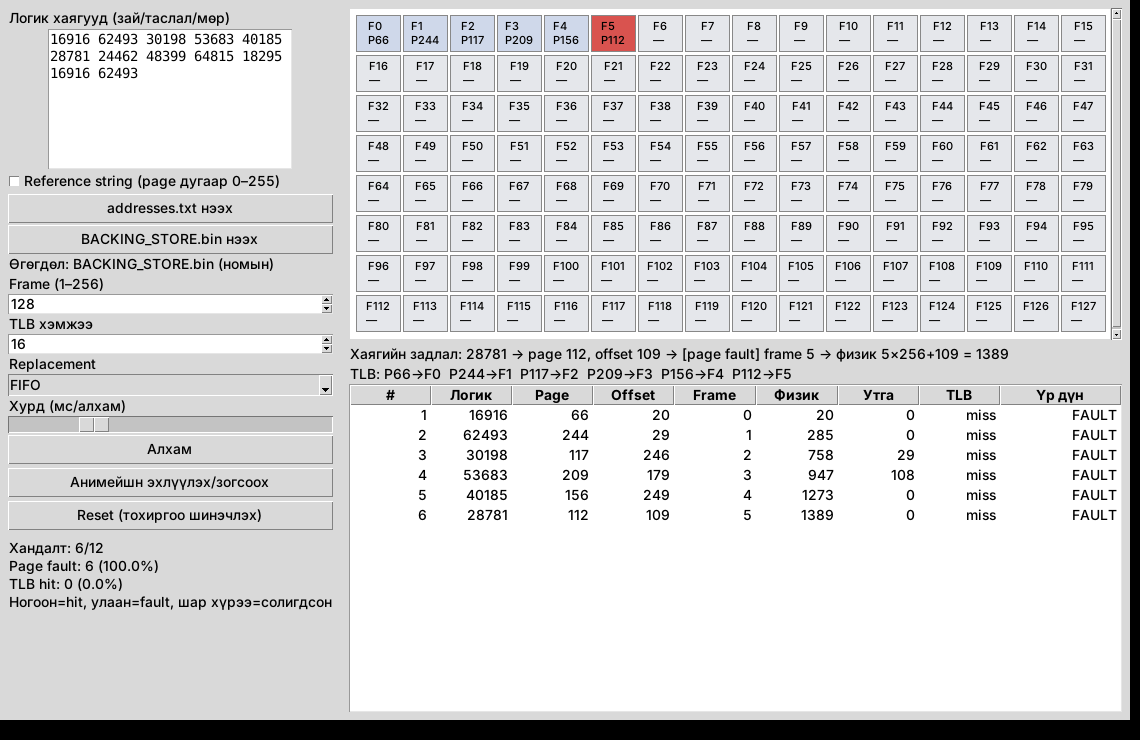
\includegraphics[width=0.74\linewidth]{gui_fault.png}
\caption{Програмын үндсэн цонх: анхдагч 12 хаяг, 128 frame, 6 дахь алхам (улаан = page fault)}\end{figure}

\subsection{Жишээнүүд}
\subsubsection{Жишээ 1. Сурах бичгийн FIFO/LRU жишээ}
\begin{enumerate}
\item \textbf{addresses.txt нээх} дарж \texttt{examples/ref\_textbook.txt}-г сонгоно.
\item \textbf{Reference string}-ийг чагтлаад Frame = \textbf{3}, Replacement = \textbf{FIFO} болгож \textbf{Reset} дарна.
\item \textbf{Анимейшн} дарж дуустал ажиллуулна → \textbf{Page fault: 15 (75.0\%)}. 4 дэх алхамд P7 гарч шар хүрээ харагдана.
\item Replacement-ийг \textbf{LRU} болгож Reset хийгээд дахин ажиллуулна → \textbf{Page fault: 12 (60.0\%)}.
\end{enumerate}
\begin{figure}[H]\centering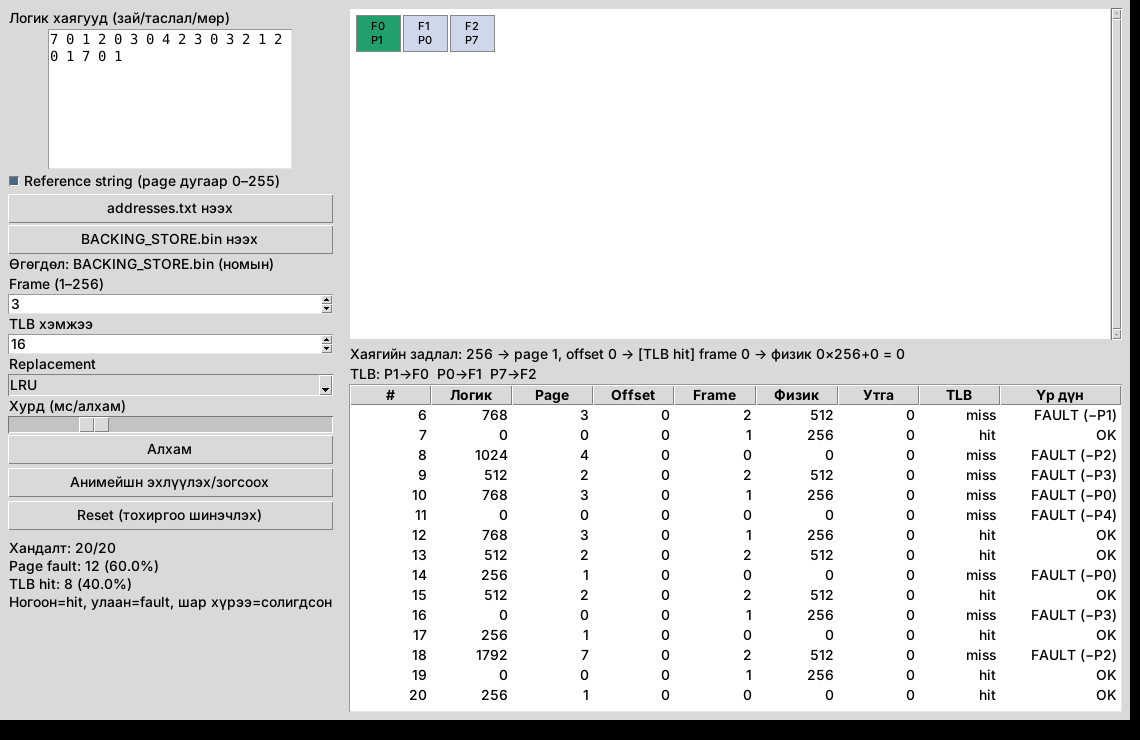
\includegraphics[width=0.72\linewidth]{gui_lru.png}
\caption{Жишээ 1: LRU, 3 frame — 20 хандалтаас 12 page fault}\end{figure}

\subsubsection{Жишээ 2. Санах ой дүүрэх ба LRU-гийн давуу тал}
\begin{enumerate}
\item \texttt{examples/addresses\_1000\_locality.txt}-г нээж, Frame = \textbf{16}, Replacement = \textbf{LRU} болгож Reset дарна.
\item Хурдыг 50 мс болгож анимейшн ажиллуулна. Эхэндээ улаан (fault) олон гарч, frame дүүрсний дараа шар хүрээтэй солилт болон ногоон hit давамгайлна.
\item Дууссаны дараа: Page fault \textbf{226 (22.6\%)}, TLB hit 774. FIFO-гоор дахин ажиллуулбал \textbf{277 (27.7\%)}.
\end{enumerate}

\subsubsection{Жишээ 3. Алдаатай оролт}
Логик хаягийн талбарт \texttt{16916 abc -5 99999999999} гэж бичээд Reset дарна. Алдаатай утга бүрийг дугаар болон шалтгааны хамт харуулсан цонх гарна (Зураг 3).
\begin{figure}[H]\centering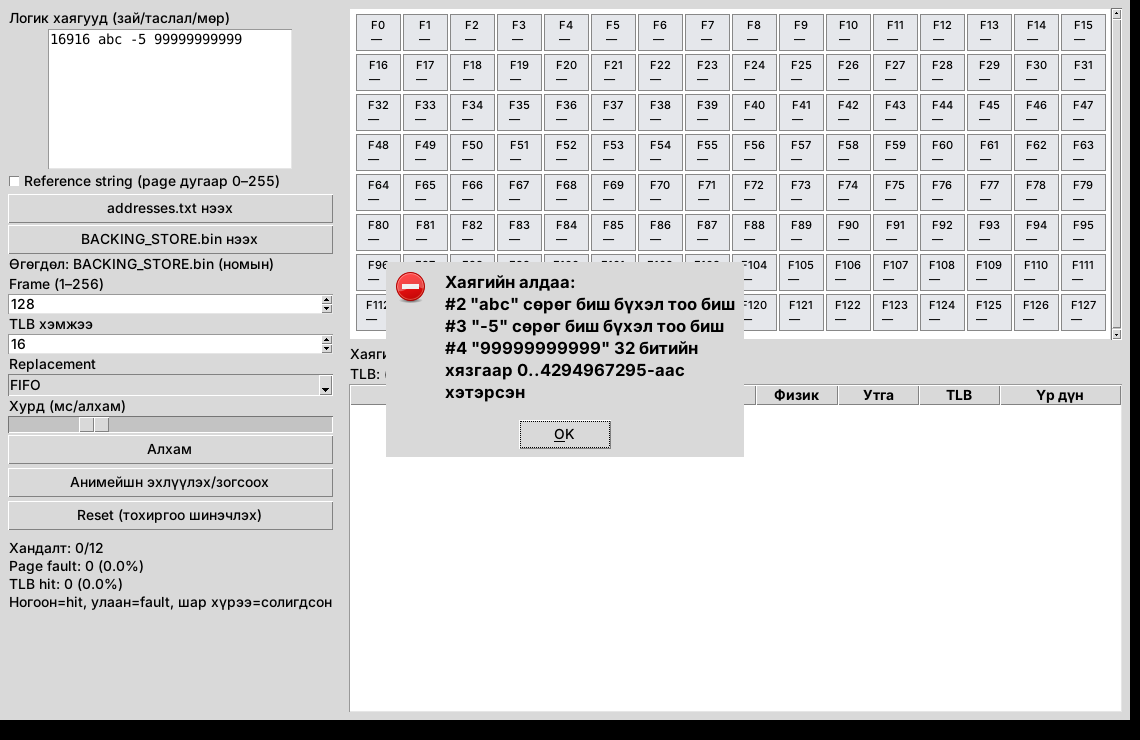
\includegraphics[width=0.66\linewidth]{gui_error.png}
\caption{Жишээ 3: алдаатай оролтын мэдэгдэл}\end{figure}

\subsubsection{Жишээ 4. Консол (CLI)}
\begin{lstlisting}
python3 src/cli.py examples/book/addresses.txt --store examples/book/BACKING_STORE.bin
python3 src/cli.py examples/ref_belady.txt --refs --frames 4 --policy FIFO --summary
python3 src/experiment.py examples/addresses_1000_locality.txt --csv result.csv
python3 tools/check_correct.py            # номын correct.txt-тэй харьцуулна
\end{lstlisting}
\begin{tabularx}{\linewidth}{@{}>{\raggedright\arraybackslash}p{4.2cm}Y@{}}
\hdr\hc{Сонголт}&\hc{Утга}\\
\texttt{--frames N}&Frame 1..256 (анхдагч 256)\\
\texttt{--policy FIFO|LRU}&Replacement (анхдагч FIFO)\\
\texttt{--tlb N}&TLB хэмжээ (анхдагч 16)\\
\texttt{--store FILE}&BACKING\_STORE.bin\\
\texttt{--refs}&Файлын тоонуудыг page дугаар гэж үзэх\\
\texttt{--summary}&Зөвхөн статистик хэвлэх\\
\end{tabularx}

\subsection{Түгээмэл алдаа ба шийдэл}
{\small
\begin{tabularx}{\linewidth}{@{}>{\raggedright\arraybackslash}p{5.4cm}>{\raggedright\arraybackslash}p{3.6cm}Y@{}}
\hdr\hc{Алдаа / шинж тэмдэг}&\hc{Шалтгаан}&\hc{Шийдэл}\\
\texttt{No module named 'tkinter'}&tkinter суугаагүй&Linux: \texttt{sudo apt install python3-tk}. Windows: python.org суулгацад „tcl/tk and IDLE“-г чагтлах\\
\texttt{'python3' is not recognized}&Windows дээр PATH-д байхгүй&\texttt{py src\textbackslash gui.py} эсвэл Python-ийг PATH-д нэмэх\\
\texttt{\#3 "abc" сөрөг биш бүхэл тоо биш}&Хаяг тоо биш&Зөвхөн сөрөг биш бүхэл тоо (hex, бутархай болохгүй)\\
\texttt{... 32 битийн хязгаар ...}&Хаяг $> 2^{32}-1$&Утгыг багасгах\\
\texttt{... page дугаар 0..255 байх ёстой}&Reference string горимд 255-аас их тоо&Горимыг унтраах эсвэл утгыг засах\\
\texttt{Хаягийн жагсаалт хоосон байна}&Хоосон текст/файл&Хаяг оруулах\\
\texttt{Frame-ийн тоо 1..256 ...}&Frame 0 эсвэл $>256$&1–256 утга оруулах\\
\texttt{BACKING\_STORE 65536 байт ...}&Буруу файл&Зөв BACKING\_STORE.bin сонгох\\
Тохиргоо өөрчилсөн ч үр дүн өөрчлөгдөхгүй&Reset дараагүй&\textbf{Reset} дарах\\
„Value“ нь номын correct.txt-тэй таарахгүй&CLI-д \texttt{--store} өгөөгүй (жишиг өгөгдөл)&\texttt{--store examples/book/BACKING\_STORE.bin}\\
\end{tabularx}}

% ===============================================================
\section{Operational заавар}
\subsection{Repository clone хийх}
\begin{lstlisting}
git clone https://github.com/ws202-gg/Designing-a-Virtual-Memory-Manager.git
cd Designing-a-Virtual-Memory-Manager
git checkout v1.0          # 9-р долоо хоногт нийтэлсэн хувилбар
\end{lstlisting}

\subsection{OS, compiler/runtime, version}
\begin{tabularx}{\linewidth}{@{}>{\raggedright\arraybackslash}p{3.4cm}YY@{}}
\hdr\hc{Зүйл}&\hc{Шаардлага}&\hc{Баталгаажуулсан орчин}\\
OS&Windows 10+, Linux, macOS&Ubuntu 24.04\\
Runtime&Python 3.10+&Python 3.12.3, 3.13\\
GUI&tkinter (Tk 8.6)&Tk 8.6, Xvfb (virtual display)\\
Build tool&Шаардлагагүй (interpreted)&—\\
Git&Clone хийхэд&git 2.x\\
\end{tabularx}
\begin{lstlisting}
python3 --version                                        # 3.10+
python3 -c "import tkinter; print(tkinter.TkVersion)"    # 8.6
\end{lstlisting}

\subsection{Dependency суулгах}
Гадны dependency байхгүй (зөвхөн стандарт сан). Linux дээр GUI-д \texttt{sudo apt install python3-tk} хэрэгтэй. Тайлангийн PDF-ийг дахин гаргах бол XeLaTeX ба CMU фонт хэрэгтэй (\texttt{docs/latex/}, сонголттой).

\subsection{Build ба Run команд}
\begin{tabularx}{\linewidth}{@{}lYY@{}}
\hdr&\hc{Linux / macOS}&\hc{Windows (PowerShell)}\\
\textbf{Build}&шаардлагагүй&шаардлагагүй\\
\textbf{Run (GUI)}&\texttt{python3 src/gui.py}&\texttt{py src\textbackslash gui.py}\\
\textbf{Run (CLI)}&\texttt{python3 src/cli.py <файл> [...]}&\texttt{py src\textbackslash cli.py <файл> [...]}\\
\textbf{Туршилт}&\texttt{python3 src/experiment.py <файл>}&\texttt{py src\textbackslash experiment.py <файл>}\\
\textbf{Автомат тест}&\texttt{python3 -m unittest discover tests -v}&\texttt{py -m unittest discover tests -v}\\
\textbf{Өгөгдөл үүсгэх}&\texttt{python3 tools/gen\_examples.py}&\texttt{py tools\textbackslash gen\_examples.py}\\
\textbf{correct.txt шалгах}&\texttt{python3 tools/check\_correct.py}&\texttt{py tools\textbackslash check\_correct.py}\\
\end{tabularx}
Repository бүтэц:
\begin{lstlisting}
Designing-a-Virtual-Memory-Manager/
|-- README.md                Төслийн нэр, код, зорилго, Quick Start
|-- src/                     vmm.py  cli.py  gui.py  experiment.py
|-- tests/test_vmm.py        24 автомат тест
|-- examples/                Өөрсдийн тестийн өгөгдөл
|   `-- book/                Номын addresses.txt, BACKING_STORE.bin, correct.txt
|-- tools/check_correct.py   correct.txt-тэй харьцуулагч
|-- tools/gen_examples.py    Туршилтын өгөгдөл үүсгэгч (seed=2026)
`-- docs/                    Report.pdf, Manual.pdf, img/, results/*.csv, latex/
\end{lstlisting}

\subsection{Үндсэн тестийн өгөгдөл ба хүлээгдсэн үр дүн}
\texttt{python3 -m unittest discover tests -v} → \texttt{Ran 24 tests ... OK}. Номын албан ёсны өгөгдлөөр шалгах ба CLI-ийн үндсэн туршилтууд. \texttt{examples/}-ээр эхэлсэн мөрүүдийн урд \texttt{python3 src/cli.py} нэмж ажиллуулна:

{\small
\begin{tabularx}{\linewidth}{@{}>{\raggedright\arraybackslash}p{8.3cm}Y@{}}
\hdr\hc{Команд}&\hc{Хүлээгдсэн үр дүн}\\
\textbf{\texttt{python3 tools/check\_correct.py}}&\texttt{1000/1000 мөр таарсан ... Page Faults = 244, TLB Hits = 54}\\
\textbf{\texttt{python3 tools/check\_correct.py --frames 128 --policy LRU}}&\texttt{1000/1000 утга (Value) таарсан ... Page Faults = 539}\\
\texttt{examples/addresses.txt --frames 128}&10 мөр. Эхнийх нь \texttt{Virtual address: 16916 Physical address: 20}. \texttt{Page Faults = 10}, \texttt{TLB Hits = 0}\\
\texttt{examples/ref\_textbook.txt --refs --frames 3 --policy FIFO --summary}&\texttt{Page Faults = 15}\\
\texttt{examples/ref\_textbook.txt --refs --frames 3 --policy LRU --summary}&\texttt{Page Faults = 12}\\
\texttt{examples/ref\_belady.txt --refs --frames 3 --summary}&\texttt{Page Faults = 9}\\
\texttt{examples/ref\_belady.txt --refs --frames 4 --summary}&\texttt{Page Faults = 10} (Belady)\\
\texttt{examples/addresses\_1000\_locality.txt --frames 16 --policy LRU --summary}&\texttt{Page Faults = 226}, \texttt{TLB Hits = 774}\\
\texttt{examples/addresses\_1000\_locality.txt --frames 16 --policy FIFO --summary}&\texttt{Page Faults = 277}, \texttt{TLB Hits = 723}\\
\end{tabularx}}

\subsection{Нэмэлт boundary / error тест}
{\small
\begin{tabularx}{\linewidth}{@{}>{\raggedright\arraybackslash}p{6.6cm}Y@{}}
\hdr\hc{Команд (\texttt{python3 src/cli.py ...})}&\hc{Хүлээгдсэн үр дүн}\\
\texttt{examples/boundary.txt --frames 128}&65535 → physical 767, 65536 → physical 0. \texttt{Page Faults = 3}, \texttt{TLB Hits = 4}\\
\texttt{examples/addresses.txt --frames 1 --policy LRU}&\texttt{Page Faults = 10}. Хандалт бүрт өмнөх page гарна\\
\texttt{examples/bad\_input.txt}&\texttt{Алдаа: Хаягийн алдаа: \#2 "abc" ...}. Exit code 2\\
\texttt{examples/empty.txt}&\texttt{Алдаа: Хаягийн файл хоосон байна}. Exit 2\\
\texttt{examples/addresses.txt --frames 0}&\texttt{Frame-ийн тоо 1..256 ...}. Exit 2\\
\texttt{missing.txt}&\texttt{... файлыг нээж чадсангүй ...}. Exit 2\\
\end{tabularx}}
Exit code шалгах: Linux/macOS \texttt{echo \$?}, Windows PowerShell \texttt{\$LASTEXITCODE}.

\subsection{Known issues}
\begin{itemize}
\item CLI-д \texttt{--store} өгөхгүй бол „Value“ нь жишиг өгөгдлийн утга байна (хаяг хөрвүүлэлт, fault, TLB-ийн статистикт нөлөөгүй). Номын утгыг авахын тулд \texttt{--store examples/book/BACKING\_STORE.bin} өгнө.
\item TLB-ийн replacement нь page replacement-тэй ижил бодлого ашигладаг (тусад нь сонгох боломжгүй).
\item Write/dirty bit, олон процесс хэрэгжээгүй.
\item Тохиргоо өөрчлөхөд Reset дарах шаардлагатай (Reference string чагтлахаас бусад үед).
\item Маш олон хаягтай (10\,000+) жагсаалтыг GUI-д ачаалахад хүснэгт удааширч болно. Ийм үед CLI-г ашиглана.
\end{itemize}
\end{document}
